\documentclass[border=10pt]{standalone}
\usepackage{tikz}\usepackage{amsmath}\usetikzlibrary{arrows.meta}
\begin{document}
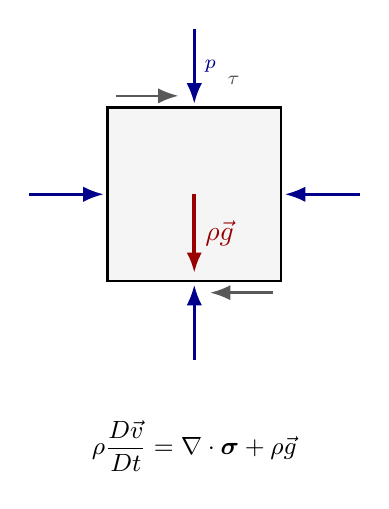
\begin{tikzpicture}[line width=0.9pt,>={Latex[length=2.6mm]}]
  \draw[fill=black!4] (0,0) rectangle (2.2,2.2);
  % presion (normal, hacia adentro)
  \draw[->,blue!55!black] (1.1,3.2)--(1.1,2.25) node[midway,right]{\scriptsize$p$};
  \draw[->,blue!55!black] (1.1,-1.0)--(1.1,-0.05);
  \draw[->,blue!55!black] (-1.0,1.1)--(-0.05,1.1);
  \draw[->,blue!55!black] (3.2,1.1)--(2.25,1.1);
  % cortantes viscosos (tangenciales)
  \draw[->,black!65] (0.1,2.35)--(0.9,2.35); \draw[->,black!65] (2.1,-0.15)--(1.3,-0.15);
  \node[black!65] at (1.6,2.55){\scriptsize$\tau$};
  % fuerza masica
  \draw[->,red!60!black,line width=1.3pt] (1.1,1.1)--(1.1,0.1) node[midway,right]{$\rho\vec g$};
  \node[align=center] at (1.1,-2.1){\small $\rho\dfrac{D\vec v}{Dt}=\nabla\cdot\boldsymbol\sigma+\rho\vec g$};
\end{tikzpicture}
\end{document}
